\documentclass[output=paper, 
colorlinks,
citecolor=brown,
newtxmath
]{langscibook} 
\bibliography{localbibliography}

\author{Rafael Ignacio Zurita\affiliation{Universidad Nacional del Comahue}}
\title{Herramientas de desarrollo}  
\abstract{
En este capítulo se examinan los pasos involucrados en la preparación
del software para un sistema embebido, y de las
las herramientas de desarrollo asociadas al proceso.
Se proporciona, como ejemplo, la
construcción del programa \textit{LED blink} que es analizado en detalle
en el siguiente capítulo.

Nos enfocaremos unicamente en el uso de las herramientas open source 
provistas por GCC (the GNU Compiler Collection), las cuales son 
parte del proyecto GNU.


\keywords{sistema embebido, ciclo de compilación, GNU GCC, compiladores cruzados (cross-compilers), cadena de desarrollo (toolchains)}
}



% add all extra packages you need to load to this file  
\usepackage{tabularx} 

%%%%%%%%%%%%%%%%%%%%%%%%%%%%%%%%%%%%%%%%%%%%%%%%%%%%
%%%                                              %%%
%%%           Examples                           %%%
%%%                                              %%%
%%%%%%%%%%%%%%%%%%%%%%%%%%%%%%%%%%%%%%%%%%%%%%%%%%%% 
%% to add additional information to the right of examples, uncomment the following line
% \usepackage{jambox}
%% if you want the source line of examples to be in italics, uncomment the following line
% \renewcommand{\exfont}{\itshape}
% \usepackage{./langsci/styles/jambox}
\usepackage{./langsci/styles/langsci-lgr}
\usepackage{./langsci/styles/langsci-osl}
\usepackage{langsci-optional}
% \usepackage{langsci-gb4e}
\usepackage{langsci-cgloss}

\usepackage[linguistics]{forest}

\makeatletter
\let\thetitle\@title
\let\theauthor\@author 
\makeatother

\newcommand{\togglepaper}[1][0]{ 
%   \bibliography{../localbibliography}
  \papernote{\scriptsize\normalfont
Esta es una obra derivada oficialmente autorizada por O'Reilly(*) para la materia "Programación de Sistemas Embebidos" de la Facultad de Informática, Universidad Nacional del Comahue. \\ Detalles de la autorización oficial y sus modificaciones al final del capítulo. \\ Libro original: Programming Embedded Systems with C and GNU Development Tools,
Second Edition, by Michael Barr and Anthony Massa. Copyright 2007 O'Reilly Media, Inc., 978-0-596-00983-0
%    \theauthor.
%    \thetitle. 
%    To appear in: 
%    Change Volume Editor \& in localcommands.tex 
%    Change volume title in localcommands.tex
 %   Berlin: Language Science Press. [preliminary page numbering]
  }
 % \pagenumbering{roman}
  \setcounter{chapter}{#1}
  \addtocounter{chapter}{-1}
}


\usepackage[spanish]{babel}
\usepackage[bottom]{footmisc}
\usepackage{tabularx}

\definecolor{aliceblue}{rgb}{0.94, 0.97, 1.0}

% \IfFileExists{../localcommands.tex}{%hack to check whether this is being compiled as part of a collection or standalone
%   % add all extra packages you need to load to this file  
\usepackage{tabularx} 

%%%%%%%%%%%%%%%%%%%%%%%%%%%%%%%%%%%%%%%%%%%%%%%%%%%%
%%%                                              %%%
%%%           Examples                           %%%
%%%                                              %%%
%%%%%%%%%%%%%%%%%%%%%%%%%%%%%%%%%%%%%%%%%%%%%%%%%%%% 
%% to add additional information to the right of examples, uncomment the following line
% \usepackage{jambox}
%% if you want the source line of examples to be in italics, uncomment the following line
% \renewcommand{\exfont}{\itshape}
% \usepackage{./langsci/styles/jambox}
\usepackage{./langsci/styles/langsci-lgr}
\usepackage{./langsci/styles/langsci-osl}
\usepackage{langsci-optional}
% \usepackage{langsci-gb4e}
\usepackage{langsci-cgloss}

\usepackage[linguistics]{forest}

%   \makeatletter
\let\thetitle\@title
\let\theauthor\@author 
\makeatother

\newcommand{\togglepaper}[1][0]{ 
%   \bibliography{../localbibliography}
  \papernote{\scriptsize\normalfont
Esta es una obra derivada oficialmente autorizada por O'Reilly(*) para la materia "Programación de Sistemas Embebidos" de la Facultad de Informática, Universidad Nacional del Comahue. \\ Detalles de la autorización oficial y sus modificaciones al final del capítulo. \\ Libro original: Programming Embedded Systems with C and GNU Development Tools,
Second Edition, by Michael Barr and Anthony Massa. Copyright 2007 O'Reilly Media, Inc., 978-0-596-00983-0
%    \theauthor.
%    \thetitle. 
%    To appear in: 
%    Change Volume Editor \& in localcommands.tex 
%    Change volume title in localcommands.tex
 %   Berlin: Language Science Press. [preliminary page numbering]
  }
 % \pagenumbering{roman}
  \setcounter{chapter}{#1}
  \addtocounter{chapter}{-1}
} 
%\togglepaper[1]
% }{}

\begin{document}

\selectlanguage{spanish}

\chapterfont{\Large\color{LightBlue}} 
%\chapternumberfont{\large} 
%\chaptertitlefont{\Large}
\chapter*{1 Programación de Sistemas Embebidos 2020\\ Herramientas de desarrollo}
esta es una prueba
{\def\addcontentsline#1#2#3{}\maketitle}

\chapter*{Programación de Sistemas Embebidos 2020\\ Herramientas de desarrollo}

\begingroup
\let\clearpage\relax
\cleardoublepage
\hypersetup{linkcolor=blue}
\tableofcontents*
\endgroup


\footnote{\scriptsize\normalfont Esta es una obra derivada oficialmente autorizada por O'Reilly(*) para la materia "Programación de Sistemas Embebidos" de la Facultad de Informática, Universidad Nacional del Comahue. \\ Detalles de la autorización oficial y sus modificaciones al final del capítulo. \\ Libro original: Michael Barr. Programming Embedded Systems in C and C++. ISBN-13: 978-1565923546
ISBN-10: 1565923545. O'Reilly }

{\def\addcontentsline#1#2#3{}\maketitle}


\setcounter{page}{1}


\hfill\begin{minipage}{0.8\linewidth} \footnotesize
I consider that the golden rule requires that if I like a program I 
must share it with other people who like it. 
Software sellers want to divide the users and conquer them, making 
each user agree not to share with others. I refuse to break solidarity 
with other users in this way. I cannot in good conscience sign a
nondisclosure agreement or a software license agreement. 
So that I can continue to use computers
without dishonor, I have decided to put together a sufficient body of free software so that I will be able
to get along without any software that is not free.\\
—Richard Stallman 27-sep-1983, Founder of the GNU Project.
\end{minipage}

% \togglepaper[0]

\section {El ciclo de compilación de software}

La programación de sistemas embebidos, en una visión conceptual de alto nivel, 
no es muy diferente a la programación realizada para un programa de PC. Lo único que 
cambia en el proceso es 
que se necesita entender la plataforma de hardware destino para poder compilarlo. 
Desafortunadamente, cada plataforma de hardware es única, aún cuando
todas las plataformas de hardware embebido contienen los mismos periféricos
básicos más una CPU y memorias. Cada ínfimo detalle de bajo nivel de estos 
componentes son diferentes. Por ejemplo, el método de configuración
de los registros de control
de una interfaz serial puede variar de procesador a procesador 
y de plataforma a plataforma.
Estas diferencias entre las plataformas de hardware
agrega una complejidad adicional, y es también la razón
por la cual se necesita trabajar más que antes en el proceso 
de construcción del software embebido.

\subsection {Cadena de herramientas (toolchains)}

Cuando las herramientas de desarrollo se utilizan en el mismo sistema 
donde se ejecutará el programa, el compilador y programas asociados
pueden realizar varias suposiciones sobre el sistema automáticamente.
No es el caso en el desarrollo de sistemas embebidos, donde las herramientas
de desarrollo se ejecutan en una máquina (host) diferente a la plataforma
de hardware destino (target). En este último caso, el usuario debe proveer 
conocimiento del sistema a las herramientas, a través 
de una mayor cantidad de instrucciones explícitas que lo que haría
si tanto el target como el host fueran la misma plataforma.

 
\begin{center}
\begin{tabularx}{0.95\textwidth}{|X|}
\hline
\rowcolor{aliceblue}
\textbf{Target platform}\\ \\
La plataforma destino (target) incluye tanto el hardware como así
también el sistema operativo, que conforman el ambiente de ejecución
básico para la aplicación. Si no existe sistema operativo, como es
muchas veces el caso en sistemas embebidos, la plataforma destino
es simplemente el procesador en el cual se ejecuta el  programa.\\
\hline
\end{tabularx}
\end{center}

\subsubsection{Definiciones}

Al conjunto de programas que se utilizan para convertir un
archivo de código fuente a un programa ejecutable se lo denomina
\textit{\textbf{toolchain (cadena de herramientas)}}. Algunas veces
se lo denomina de manera resumida \textit{compilador}, pero recordemos
que el compilador unicamente \textit{traduce} el código fuente 
a un código en lenguaje ensamblador (luego se necesita un ensamblador
y otras herramientas como se detalla en las siguientes secciones).

Si el desarrollo del sistema se realiza en la misma máquina
donde se ejecutará el programa final, entonces el compilador es un compilador 
nativo (\textit{\textbf{native compiler}}),
al igual que el resto de las herramientas 
(\textit{\textbf{native toolchain}}).

En cambio, si el desarrollo del sistema embebido se realiza en una PC
(u otra computadora diferente al hardware destino) el compilador
es un \textit{\textbf{compilador cruzado (cross-compiler)}}, y el resto
de los programas para desarrollo conforman las \textit{\textbf{herramientas
de desarrollo cruzadas (cross-toolchain)}}.

Por lo tanto, si usted compila un programa en lenguaje C y lo ejecuta
en su PC, tanto el compilador como el programa ejecutable son nativos.
Pero, si se desarrolla un programa en C para que se ejecute
en una arquitectura diferente, su PC, o computadora de desarrollo,
contendrá un segundo compilador, el cual será un compilador cruzado.
En el caso de usar compiladores del proyecto GCC, usualmente 
se tiene un compilador de C llamado gcc (compilador nativo para ejecutar
en PC y generar programas ejecutables para PC), y un segundo compilador
gcc llamado de una manera diferente (por ejemplo, mips-gcc, el cual
se utilza en PC para generar un programa ejecutable para una computadora
de arquitectura MIPS).

\subsubsection*{Componentes de un toolchain}

Los herramientas para desarrollo de software en C (toolchain) en realidad
son pocas. Para programar en lenguaje C utilizando GCC necesita :

\begin{verbatim}

- un editor de texto sencillo
- el compilador de C (gcc)
- las herramientas binutils (ensamblador as, linker ld, etc).
- la biblioteca de c (libc)

\end{verbatim}

En sistemas Linux todas estas herramientas ya vienen enpaquetadas,
y para arquitecturas diferentes. Por ejemplo, si usted quisiera programar
en C para arquitectura MIPS y AVR tendrá que instalar en un sistema Linux
típico los siguientes paquetes: 

\begin{verbatim}
Para arquitectura MIPS:
- gcc-mips: el compilador de C cruzado para mips
- binutuils-mips: las harramientas binutils para mips
- libc-mips: biblioteca estándar de C para mips

Para arquitectura AVR:
- gcc-avr: el compilador de C cruzado para avr
- binutuils-avr: las harramientas binutils para avr
- avr-libc: biblioteca estándar de C para avr
\end{verbatim}

\subsection{Ciclo de compilación}

El proceso de convertir el código fuente del software embebido
en una imagen binaria ejecutable involucra cuatro pasos bien distinguidos:

\begin{enumerate}
\item Escribir un programa en un lenguaje de programación. Si el proyecto
es de mediana complejidad entonces se escriben varios archivos fuente.
\item Cada archivo fuente debe ser compilado en un archivo objeto.
\item Todos los archivos objetos del paso dos deben ser vinculados en conjunto
(linked) para generar un archivo objeto individual, llamado el programa reubicable.
\item Direcciones físicas de la memoria deben ser asignadas a los desplazamientos (offsets)
dentro del programa reubicable en un proceso llamado reubicación (relocation).
\end{enumerate}


El proceso recién descripto está representado en la Figura \ref{fig:compilacion}.
Allí se se observan los cuatro pasos comenzado desde arriba hacia abajo,
en conjunto con las herramientas utilizadas (que aparecen
en los recuadros con esquinas redondeadas).
Estas herramientas de desarrollo toman uno o más archivos como entrada
y producen un archivo individual como salida. 
El resultado del paso final es un archivo que contiene una imagen binaria
que está lista para ser ejecutada en el sistema embebido destino.

\begin{figure}
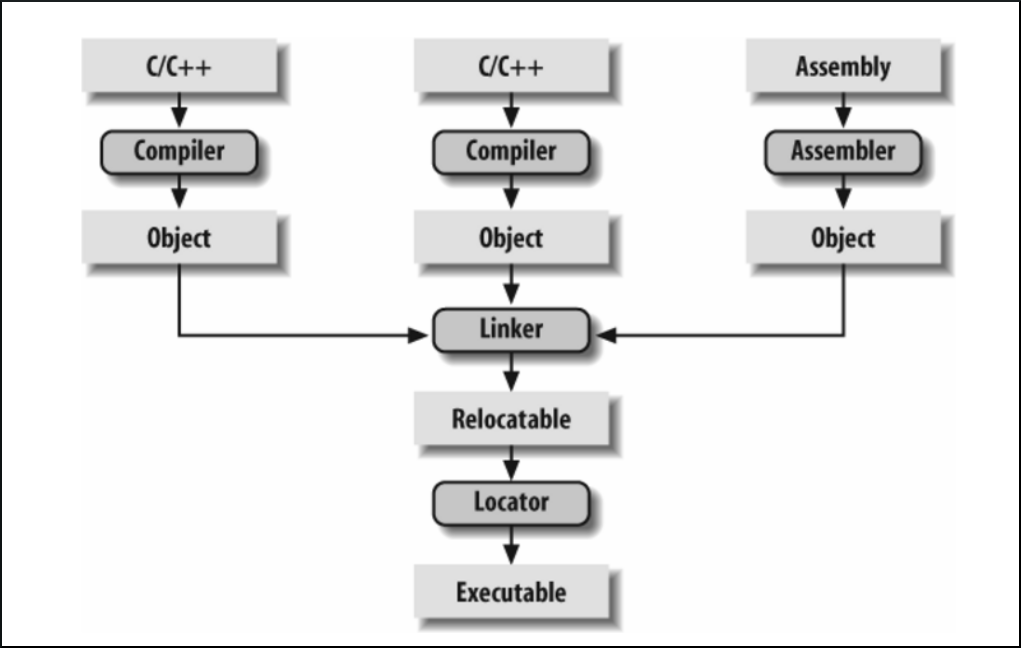
\includegraphics[width=\linewidth]{images/ciclo_de_compilacion.png}
\caption{El proceso de desarrollo de software embebido.}
\label{fig:compilacion}
\end{figure}



Cada paso del proceso de compilación de software embebido
es una transformación realizada por software ejecutado en una computadora
de propósito general. Para distinguir esta computadora de desarrollo (usualmente una 
PC o estación de trabajo UNIX) del sistema embebido destino se utiliza el término \textit{\textbf{host computer}}.
En esta computadora es donde se ejecuta el compilador, ensamblador, vinculador y se realiza la reubicación (location).
Aunque, como ya mencionado, estas herramientas trabajan en conjunto
para producir una imagen binaria que puede ser ejecutada
únicamente en el sistema embebido destino (\textit{\textbf{target
computer}}). Esta división de responsabilidades
se representan en la Figura \ref{fig:compilacion2}

\begin{figure}[H]
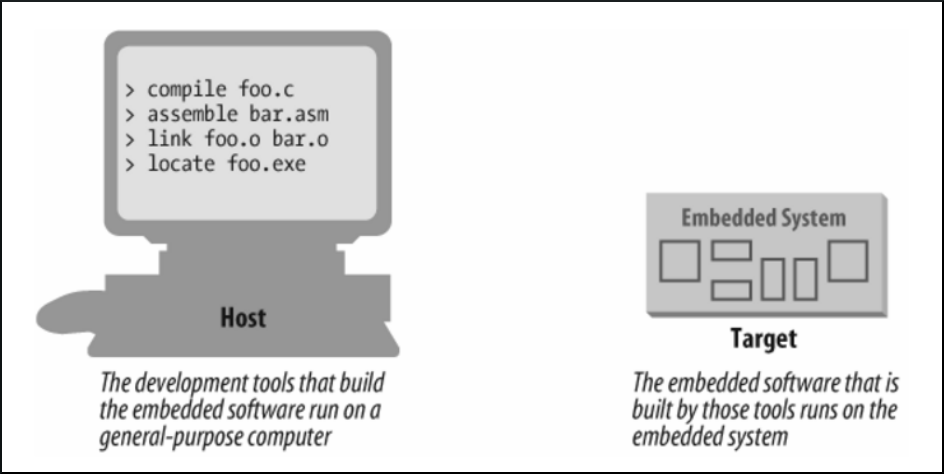
\includegraphics[width=10cm]{images/host_target.png}
\caption{Computadora de desarrollo (host) y computador destino (target).}
\label{fig:compilacion2}
\end{figure}

En este texto se utilizan las herramientas de desarrollo del proyecto GNU
(compilador, ensamblador, vinculador y debugger) las cuales son software libre
y tienen extensa documentación en libros, y páginas de manual online en sistemas
Linux y UNIX. Una vez comprendido
el uso de las mismas puede aplicarse los mismos conceptos a herramientas
de desarrollo equivalentes (comerciales o no).

\subsection {Compilando}

La tarea de un compilador es, principalmente, traducir programas escritos en 
algún lenguaje leíble por personas en un conjunto equivalente
de códigos de operación para algún procesador particular. En ese sentido,
el ensamblador es también un compilador (generalmente se lo llama
compilador de lenguaje ensamblador), pero su tarea es mas sencilla, ya que
realiza una traducción de uno a uno, de nemotécnicos leíble por personas
en sus equivalentes códigos de operación de la CPU. El resto de lo explicado en esta sección
aplica tanto a compiladores como a los ensambladores. En conjunto, 
estas herramientas realizan el primer paso del proceso de construcción 
de software de un sistema embebido.

Por supuesto, cada procesador tiene su propio lenguaje máquina, por lo que
necesita seleccionar un compilador que produzca programas para el procesador
destino específico. En el caso de los sistemas embebidos,  este compilador
casi siempre se ejecuta en la computadora host. Simplemente no tiene sentido,
la mayoría de las veces, ejecutar el compilador en el sistema embebido.
Un compilador que realiza esta tarea -se ejecuta en una plataforma  y produce
código para otra- es llamado un compilador cruzado (cross-compiler). El uso de
un compilador cruzado es una de las características de desarrollo de software
embebido.

El \textit{\textbf{compilador GNU de lenguaje C (gcc) y el ensamblador (as)}} pueden ser configurados y compilados
para que trabajen como compiladores nativos o compiladores cruzados. 
Estas herramientas soportan
un impresionante conjunto de combinaciones host-target. El compilador gcc ha sido
portado a todos los sistemas operativos Mac y PC. También, el soporte de procesadores destino
es extenso, e incluye AVR, Intel x86, MIPS, PowerPC, ARM y SPARC. Información
adicional puede ser encontrada online\footnote{\texttt{http://gcc.gnu.org}}.

Cualquiera sea el lenguaje de entrada (C, C++, ensamblador o cualquier otro), la salida
de un compilador cruzado será un \textit{\textbf{archivo objeto}}. Este es un archivo binario con
formato especial que contiene el conjunto de instrucciones y datos
resultado del proceso de traducción del lenguaje. Aunque partes de este archivo
contiene código ejecutable \textit{el archivo objeto no puede ser ejecutado directamente}.


El contenido de un archivo objeto puede ser imaginado como una estructura de datos
muy grande y flexible. La estructura del archivo está definida en un formato estándar, 
por ejemplo, Common Object File Format (COFF) o Executable and Linkable Format (ELF).
Si se utiliza más de un compilador (i.e. se está escribiendo diferentes partes de un programa
en diferentes lenguajes fuente) se debe estar seguro que el compilador es capaz
de producir archivos objetos en el mismo formato. En este contexto, gcc soporta 
los dos formatos recién mencionados. Aunque muchos compiladores (y en particular
los que son para ambientes UNIX) soportan formatos de archivo objeto como
COFF y ELF, algunos producen archivos objetos en formatos propietarios.
Si se utilizan compiladores de este último grupo se necesita obtener todas
las herramientas de desarrollo restantes desde el mismo proveedor.

\subsubsection*{Estructura de un archivo objeto}
La mayoría de los archivos objetos comienzan con un encabezado que describe las secciones
que siguen. Cada una de esas secciones contienen uno o mas bloques de código o datos que 
provienen de los archivos fuentes. De cualquier manera, el compilador tiene reagrupado
esos bloques en secciones relacionadas. Por ejemplo, gcc agrupa todos los bloques de
código en una sección llamada text, todas las variables globales inicializadas (y sus
valores iniciales) en una sección llamada data, y todas las variables globales sin 
inicializar en una sección llamada bss.

Usualmente, existe también una tabla de símbolos en el archivo objeto, que contiene
los nombres y las ubicaciones de todas las variables y funciones referenciadas dentro
del archivo fuente. Partes de esta tabla podría estar incompleta, debido a que
no todas las variables y funciones son siempre definidas en el mismo archivo fuente. 
Esos son los símbolos que hacen referencia a variables y funciones definidas en 
otro archivo fuente distinto. Es trabajo del vinculador resolver todas esas referencias
no resueltas. Si se necesita revisar la tabla de símbolos de un archivo objeto
o ejecutable puede utilizar la herramienta \textit{\textbf{objdump}} del paquete binutils.
Por ejemplo, con el argumento -t :

\begin{verbatim}
# objdump -t  main.o
\end{verbatim}

\subsection {Vinculando}

Todos los archivos objetos que fueron el resultado del paso dos del proceso deben
ser vinculados. Los archivos objetos individualmente están incompletos, por lo que
alguna de las referencias a variables y funciones internas aún no han sido resueltas.
La tarea del vinculador (linker) es combinar esos archivos objetos, y en el proceso,
resolver todos los símbolos no resueltos. La salida del vinculador es un nuevo archivo objeto, que contiene todo el código y datos
de los archivos objetos de entrada (en el mismo formato).
Eso es logrado al combinar las secciones text, data y bss de los archivos de entrada.
Cuando el vinculador finaliza, todo el código en lenguaje máquina de todos los archivos
objetos de entrada está en la sección text del nuevo archivo, y todas las variables
inicializadas o no en las secciones nuevas data y bss respectivamente.

Mientras el vinculador está en el proceso de integrar 
los contenidos de las secciones también 
busca los símbolos sin resolver. Por ejemplo, si un archivo objeto contiene 
una referencia no resuelta a  una variable llamada \textit{foo}, y una variable con 
el mismo nombre está declarada en uno de los archivos objetos, el vinculador
integrará ambas. La referencia no resuelta sera reemplazada con la referencia
a la variable encontrada. Por ejemplo, si \textit{foo} está ubicada a 14 bytes de desplazamiento
de donde comienza la sección de datos, su entrada en la tabla de símbolos ahora
contendrá esa dirección.

El \textit{\textbf{vinculador de GNU (ld)}} está portado a todas las mismas plataformas en donde
fue portado el compilador GNU (gcc). Esta es una herramienta de la linea de comandos
que toma como argumentos de entrada todos los nombres de los archivos objeto, 
y posiblemente bibliotecas a ser vinculadas.
Cuando se desarrolla software embebido, un archivo objeto especial que contiene el \textit{\textbf{código de 
inicialización (startup code)}}, debe también ser incluido dentro de esta
lista de archivos que procesa ld (se darán mas detalles sobre el código
de inicialización en secciones siguientes). Este código de startup
tambien se utiliza al programar para una PC, sólo que el compilador nativo
ya conoce cuál es automáticamente. Finalmente, cabe mencionar
que el vinculador GNU tiene un lenguaje de scripting que puede ser utilizado
para controlar cómo debe ser el archivo objeto de salida si se requiere.

Si el mismo símbolo es declarado en más de un archivo objeto de los que 
procesa el vinculador ld, entonces el proceso finaliza inmediatamente, y ld mostrará
un mensaje de error explicando la situación (error de programación).

\begin{center}
\begin{tabularx}{0.95\textwidth}{|X|}
\hline
\rowcolor{lightgray}
\textbf{Vinculación Estática vs Vinculación Dinámica}\\
Si una referencia a un símbolo queda sin resolver luego de
que se procesaron todos los archivos objetos, el vinculador intentará 
resolver la misma por su cuenta.
La referencia podría ser una función, tal como memcpy, strlen o malloc, que son
parte de la biblioteca estándar de C, por lo que ld abrirá cada uno de las
bibliotecas descriptas como argumentos en la línea de comandos (en el orden
en que se mencionaron) y examina sus tablas de símbolos. 
Si el vinculador descubre una función o variable con ese nombre la referencia
será resuelta agregando el código y datos asociados a esta referencia en el 
archivos objeto de salida (en una \textbf{compilación estática}, lo cual es
frecuente en sistemas embebidos sin sistema operativo). 
Cuando se realiza \textbf{vinculación dinámica} de bibliotecas, el código 
y datos asociados con la rutina de la biblioteca no son insertadas dentro
del programa, ya que se cargan dinámicamente con asistencia
del sistema operativo, y son bibliotecas compartidas entre todos
los programas en ejecución que las utilicen.\\
\hline
\end{tabularx}
\end{center}

\begin{center}
\begin{tabularx}{\textwidth}{|X|}
\hline
\rowcolor{lightgray}
\textbf{Vinculación selectiva}\\
Si el vinculador GNU ld encuentra funciones sin referenciar en el código
(es decir, son funciones que no se utilizan), entonces ld descarta ese código y lo deja
afuera de la imagen de salida resultante.\\
\hline
\end{tabularx}
\end{center}

\subsubsection*{Biblioteca estándar de C para embebidos}

Las rutinas de la biblioteca estándar de C algunas veces requieren 
algunos o varios cambios antes que puedan ser utilizada en un sistema 
embebido nuevo.

Un problema es que las bibliotecas estándar provistas comercialmente
con la mayoría de las 
suites de herramientas de desarrollo de software propietarias
vienen únicamente en forma de archivo objeto.
Rara vez se tiene acceso al código fuente de la biblioteca para hacer los 
cambios necesarios. Por suerte, si ese es su caso, existen algunas 
alternativas. 

Una de ellas es
la provista por la compañía Cygnus (ahora parte de Red Hat),
la cual creó una versión libre de la biblioteca estándar de C para utilizar 
en sistemas embebidos.
Este paquete es llamado \textit{\textbf{newlib}}. Simplemente se necesita descargar el código fuente
para esta biblioteca desde la web\footnote{\texttt{http://sourceware.org/newlib}},
implementar unas pocas funciones especificas para el hardware destino y compilar.
La biblioteca puede luego ser vinculada con nuestras aplicaciones embebidas
para resolver cualquier llamada a la biblioteca estándar sin 
resolver previamente. 

Afortunadamente, para la arquitectura de microcontroladores AVR en particular, 
existe una versión open source de la biblioteca estándar de C, llamada 
\textit{\textbf{avr-libc}}\footnote{\texttt{https://www.nongnu.org/avr-libc/}}. 
El inicio de su sitio web,
(el cual provee la biblioteca y su documentación) puede verse en la Figura \ref{fig:avr_libc}.


\begin{figure}[H]
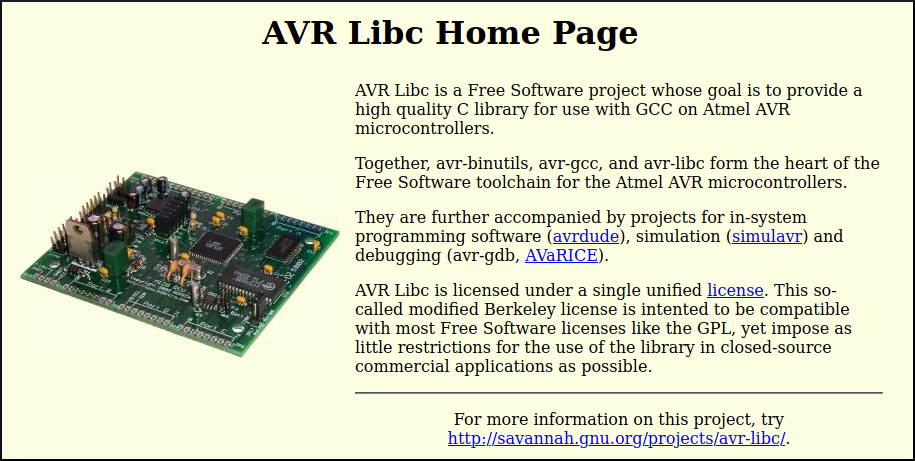
\includegraphics[width=12cm]{images/avr-libc2.png}
\caption{AVR-Libc Home Page}
\label{fig:avr_libc}
\end{figure}


Luego de integrar todas las secciones de código y datos, y de resolver todas
las referencias a símbolos, el vinculador genera un archivo objeto que es
una copia especial \textit{reubicable (relocatable)} del programa. 
En otras palabras,
el programa ya está completo, con la excepción de una cosa: todavía
resta definir las direcciones de memoria asignadas a las secciones de código y 
datos. Si no se estuviera realizando el proceso para ejecutarse en un 
sistema embebido entonces el programa estaría listo para ejecutarse.

Pero, los programadores de sistemas embebidos aún deben realizar una
tarea más en este punto, ya que 
las direcciones de los símbolos en el proceso de vinculación son relativas.
Aun si su sistema embebido incluye un sistema operativo, es necesario
que la imagen binaria final sea ubicada de manera absoluta (y no relativa).
De hecho, si existe un sistema operativo en el proyecto del sistema embebido,
el código y datos del mismo son parte del programa reubicable 
también.
La aplicación embebida completa -incluyendo el sistema operativo- es
frecuentemente vinculada en conjunto y ejecutada como una imagen binaria
individual. A esta imagen se la denomina comunmente \textit{\textbf{firmware}}.

\subsubsection {Código de inicialización (Startup code)}

Una de las acciones que las herramientas de software tradicional realizan
es agregar automáticamente el código de inicialización: un pequeño bloque
de código en lenguaje ensamblador que prepara el ambiente para la ejecución
del software escrito en un lenguaje de alto nivel. Cada lenguaje de alto
nivel tiene un conocimiento propio acerca del ambiente de ejecución.
Por ejemplo, los programas escritos en C utilizan una pila (stack). El espacio
para la pila tiene que ser reservado y ubicado antes de que el software escrito
en C pueda ser ejecutado apropiadamente. Esa es una de las responsabilidades
asignadas al código de inicialización para programas en C.

La mayoría de los compiladores cruzados (cross-compilers) para sistemas
embebidos incluyen un archivo en lenguaje ensamblador llamado startup.asm, crt0.s
(abreviatura de C runtime), o algún nombre similar. La ubicación y contenido de este
archivo está usualmente descripto en el manual suministrado con el 
compilador. El código de inicialización para programas en C usualmente 
consiste de la siguiente
lista de acciones:

\begin{enumerate}
\item Deshabilitar las interrupciones.
\item Copiar cualquier dato inicializado desde la ROM a RAM.
\item Poner en cero el área de datos sin inicializar.
\item Reservar espacio e inicializar la pila.
\item Inicializar el puntero de pila del procesador.
\item Llamar a main().
\end{enumerate}

Típicamente, el código de inicialización también incluye unas pocas
instrucciones después de llamar a main(). Estas instrucciones serán ejecutadas
sólo en el caso de que el programa en el lenguaje de alto nivel finalice (i.e.
la llamada a main retorne). Dependiendo de la naturaleza del sistema embebido
se podría utilizar estas instrucciones para realizar un halt del procesador, 
reiniciar el sistema entero, o transferir el control a una herramienta
de verificación (debug tool).

En general, el código de inicialización no es insertado automáticamente al desarrollar sistemas embebidos. El
programador debe ensamblar el código fuente del mismo e incluir el archivo objeto resultante a la 
lista de archivos de entrada del vinculador explícitamente. Además, el programador
podría necesitar indicar al vinculador una opción en la línea de comandos especial
para prevenir que ld intente insertar el código de inicialización provisto
por el toolchain.
Código de inicialización funcional para una variedad de procesadores puede
ser encontrado en el paquete GNU llamado libgloss.


\begin{center}
\begin{tabularx}{\textwidth}{|X|}
\hline
\rowcolor{lightgray}
\textbf{Debug Monitors} \\ \\
En algunos casos, un debug monitor (o ROM monitor) es el primer código
ejecutado cuando la placa es encendida. En el caso de los microcontroladores
AVR existe generalmente un bootloader que se ejecuta en primer lugar (si
el microcontrolador es complemante virgen se puede instalar un 
bootloader en caso de ser necesario).
Los bootloaders para AVR pueden ser utilizados
para descargar el firmware a través de una conexión serial, y escribir
el mismo en la memoria FLASH del microcontrolador, en la dirección 0x00.
Si el bootloader no recibe órdenes desde el puerto serial simplemente 
ejecuta la aplicación actual en FLASH.\\
\hline
\end{tabularx}
\end{center}


\subsection {Localización}

La herramienta que realiza la conversión de un programa reubicable a
una imagen binaria ejecutable es llamada \textit{\textbf{reubicador (locator)}}.
Este realiza el paso mas fácil del proceso de compilación. De hecho, 
el programador debe hacer la mayoría del trabajo en este paso, informando
detalles acerca de la memoria de la plataforma destino, como entrada.
El reubicador utiliza esta información para asignar direcciones
de memoria físicas a las secciones de código y datos dentro del programa
reubicable. Finalmente, el reubicador produce un archivo de salida que contiene
una imagen de memoria binaria que puede ser descargada dentro del sistema
embebido destino.

Cuando se escribe software para una computadora de propósito general o
sistema embebido, en algún punto las secciones del programa reubicable
deben tener asignadas direcciones concretas. Algunas veces el software
que está en la computadora destino realiza esta tarea (por ejemplo un sistema
operativo o bootloader). No es el caso más común en microcontroladores
embebidos, aunque por suerte, las herramientas de desarrollo GNU 
para arquitectura AVR traen estos detalles 
incorporadas, como así también el código de inicialización para la mayoría
de los microcontroladores de AVR de Atmel.
Cuando se realiza el paso de vinculación y localización para arquitectura AVR,
con el vinculador GNU ld, se agrega el código de inicialización y se 
resuelven las direcciones reales de acuerdo al microcontrolador destino.

En cambio, si se debe suministrar manualmente la información de la memoria 
de la plataforma destino al vinculador GNU ld, entonces se debe escribir 
un \textit{\textbf{script del vinculador (linker script)}}.
Estos scripts son utilizados algunas veces para controlar el orden exacto de
las secciones de código y datos dentro del programa reubicable, y establecer
la ubicación física de cada sección en memoria.


Debajo se muestra un ejemplo extraído y resumido de un linker script
para un microcontrolador Atmel de arquitectura AVR. El archivo script
completo es utilizado por avr-ld en la compilación del ejemplo LED blink.

\begin{verbatim}
MEMORY
{
  text   (rx)   : ORIGIN = 0, LENGTH = 8K
  data   (rw!x) : ORIGIN = 0x800100, LENGTH = 0
}
SECTIONS
{
  .text 0 :
  {
    *(.vectors)
    KEEP(*(.vectors))
     __ctors_start = . ;
     *(.ctors)
    *(.text)
  }
  .data        0 :
  {
    *(.data)
    *(.rodata)  /* We need to include .rodata here if gcc is used */
  }
  .bss  0 :
  {
    *(.bss)
    *(COMMON)
  }

...

}
\end{verbatim}

El script informa al reubicador incluido en el vinculador GNU acerca de las ubicaciones
físicas de las secciones del programa en la memoria del sistema embebido destino.
El script instruye a ld a ubicar la sección de texto en la dirección física 0x00,
y a la sección de datos en la dirección 0x800100.

Nombres en el archivo de comandos del vinculador que comienzan con un guión bajo
(ejemplo \_\_ctors\_start) pueden ser referenciado similarmente a variables ordinarias
desde dentro del código fuente en C por ejemplo. El vinculador utilizará 
estos símbolos
para resolver referencias en los archivos objeto de entrada.
Por lo que, por ejemplo, podría existir una parte del software embebido (usualmente
dentro del código de inicialización) que copia valores iniciales de las variables
inicializadas desde ROM a la sección data en RAM.

Un script para el vinculador puede también utilizar varios otros comandos
para instruir al vinculador a que realice otras operaciones.
Información adicional y opciones de los archivos script para el vinculador GNU ld
puede ser leída desde \texttt{http://www.gnu.org}.

La salida de este paso final del proceso de compilación es una imagen binaria
conteniendo direcciones físicas para el sistema embebido destino específico.
Esta imagen binaria ejecutable puede ser descargada a la memoria del sistema embebido y ejecutada.

Afortunadamente, como se mencionó anteriormente, las herramientas de desarrollo
GNU para microcontroladores AVR pueden realizar este ultimo paso automáticamente
(para casi todos lo microcontroladores existentes de esta arquitectura).

\section {Compilando el programa LED blink para una plataforma AVR}

En esta sección se muestra un ejemplo del procedimiento de compilación 
para el microcontrolador Atmel AVR atmega328p (placa arduino pro mini).
Si se utiliza otra plataforma, un proceso similar debería ser ejecutado
utilizando las herramientas y convenciones que acompañan al hardware.

\subsection {Compilar, ensamblar y vincular}

El ejemplo LED blink consiste de dos archivos fuentes : led.c y blink.c.
El primer paso en el proceso es compilar estos dos archivos.
La estructura básica para ejecutar el compilador gcc es :

\begin{verbatim}
# avr-gcc [opciones] archivo
\end{verbatim}

Compilamos y vinculamos nuestro programa con :

\begin{verbatim}
# avr-gcc -Os -DF_CPU=16000000UL -mmcu=atmega328p -c -o led.o led.c
# avr-gcc -Os -DF_CPU=16000000UL -mmcu=atmega328p -c -o blink.o blink.c
# avr-gcc -mmcu=atmega328p led.o blink.o -o led.elf
\end{verbatim}

Las opciones utilizadas son :

\begin{small}
\begin{verbatim}
-D     para definir una macro. En este caso, es una macro muy utilizada
       con el compilador avr-gcc, ya que define la velocidad del reloj del 
       microcontrolador a utilizar.
-mmcu= para seleccionar el modelo del microcontrolador destino 
-c     compilar y ensamblar, pero no vincular
\end{verbatim}
\end{small}


\begin{center}
\begin{tabularx}{\textwidth}{|X|}
\hline
\rowcolor{lightgray}
\textbf{Vinculación con gcc versus ld}\\
En el ejemplo se invoca  a gcc durante el proceso de vinculación.
Esto es debido a que el compilador gcc puede invocar al vinculador 
indirectamente.
Cuando se compila de esta manera, gcc se asegura que las versiones correctas
de ciertas bibliotecas (llamadas multilibs) sean vinculadas con llamadas
introducidas por las configuraciones del toolchain. En algunos casos, 
si el vinculador ld es invocado directamente y no gcc, el conjunto correcto de multilibs deben ser especificados en la linea de comandos, 
para asegurar que la imagen sea vinculada apropiadamente.\\
\hline
\end{tabularx}
\end{center}


El orden de los archivos objetos determinan su ubicación en memoria.
Debido a que no estamos vinculando ningún código de inicialización explícitamente
el orden de los archivos objetos es irrelevante.
Si se incluyera código de inicialización se debe ubicar el archivo objeto 
en la dirección apropiada. El archivo script para el vinculador puede ser 
utilizado para especificar donde debe residir la rutina de inicialización
en memoria. Además, puede utilizar el archivo script para 
especificar las direcciones exactas para otros código o datos, pero debe
verificar si es realmente necesario o no.

Como se observa en el comando de vinculación, los dos archivos objetos -led.o y blink.o-
son los últimos argumentos de la linea de comandos para el vinculador.
El resultado de este comando es la creación de la imagen binaria ejecutable
en formato ELF, llamada led.elf.

\subsection {Dar formato al archivo de salida}

En ciertos casos, el archivo binario ejecutable ELF producido en el 
ejemplo de la sección anterior es suficiente para descargar en el sistema 
embebido y ejecutar. En otros casos (como lo es para AVR
y su bootloader) se necesita dar formato, para la plataforma destino,
 a la imagen obtenida
en el proceso de compilación. 

Para nuestra plataforma de ejemplo necesita utilizar la herramienta
\textit{\textbf{objcopy}}, que es un programa de binutils.
objcopy es capaz de copiar el contenido de un archivo objeto en otro 
archivo objeto, pero con diferente formato.
Lo utilizaremos en nuestro ejemplo de esta manera :

\begin{verbatim}
 # avr-objcopy -O ihex -R .eeprom led.elf led.hex
\end{verbatim}

En este caso, lo utilizamos para convertir el programa LED blink
en formato ELF a una imagen en formato Intel Hex. Intel Hex 
es un formato de archivo ASCII muy utilizado en algunas plataformas
para descargar y almacenar imágenes binarias.

El comando utiliza la opción -O ihex para especificar el formato 
de archivo de salida como Intel Hex. El archivo de entrada es led.elf
y objcopy se encarga de determinar el tipo de archivo. El archivo de salida
será un nuevo archivo llamado led.hex

Algunas otras herramientas de binutils GNU son útiles para obtener 
información acerca de la imagen binaria construida.
Por ejemplo, el utilitario \textit{\textbf{size}}, el cual lista el tamaño de las secciones
para un archivo objeto. El siguiente ejemplo es presentado
para nuestro programa LED blink construido :

\begin{verbatim}
# avr-size led.elf
   text	   data	    bss	    dec	    hex	filename
    200	      0	      0	    200	     ca	led.elf
\end{verbatim}

El programa LED blink contiene 200 bytes utilizados para la sección de text 
(instrucciones máquina del programa), y
ningún byte para las secciones data y bss. La columna dec muestra el tamaño
total de la imagen, en decimal, y la columna hex en hexadecimal.


\section {Compilando el programa LED blink para una plataforma MIPS}

En esta sección se muestra un ejemplo del procedimiento de compilación 
para el procesador MIPS 24K contenido en el sistema on-chip AR9331 de atheros
(placa tplink mr3020).

\subsection {Compilar, ensamblar y vincular}

El ejemplo LED blink para MIPS consiste del archivo fuente main.c y start.S
(código de inicialización explicado en secciones anteriores).
El primer paso en el proceso es compilar estos dos archivos.
La estructura básica para el compilador gcc utilizando el toolchain openwrt
de Linaro es :

\begin{verbatim}
# mips-openwrt-linux-uclibc-gcc [opciones] archivo
\end{verbatim}

Compilamos los archivos fuentes con :

\begin{verbatim}

# mips-openwrt-linux-uclibc-gcc -O -G 0 -mno-abicalls -fno-pic \
    -Wall -DRAMSIZE=0x00100000          -mips32 -c start.S -o start.o

# mips-openwrt-linux-uclibc-gcc -O -G 0 -mno-abicalls -fno-pic \
    -Wall -DRAMSIZE=0x00100000          -mips32 -c main.c -o main.o

\end{verbatim}

Hemos realizado la compilación inicial en dos pasos, pero es posible realizar
esta acción utilizando un único comando. Ejecutar estos comandos 
permiten verificar que las herramientas de desarrollo
están instaladas y configuradas correctamente. El resultado 
de cada comando es la creación de un archivo objeto por comando, que tiene
el mismo prefijo que el archivo .c, pero con extensión .o.
Por lo tanto, si no hubieron errores en la programación, se obtiene
los archivos main.o y start.o.

\subsection {Vincular y localizar}

Ahora es el momento de realizar el segundo paso en el proceso de compilación.
Para realizar la vinculación y localización utilizaremos el vinculador GNU,
como se describió anteriormente. Tambien
utilizaremos un archivo script del vinculador, llamado
barebone.lds, que será tambien parte de la entrada a ld. Este archivo lds
permitirá establecer la ubicación de cada sección en la memoria del tplink
mr3020.  La estructura básica de este archivo, como visto antes, es :

\begin{verbatim}
# mips-openwrt-linux-uclibc-ld [opciones] archivo ...

El comando utilizado en este caso es :

# mips-openwrt-linux-uclibc-ld -o barebone.elf -Tbarebone.lds \
                -Ttext 0x80060000 start.o main.o

# mips-openwrt-linux-uclibc-objcopy -S -O srec --remove-section=.reginfo \
                --remove-section=.mdebug barebone.elf barebone.srec

# mips-openwrt-linux-uclibc-objcopy -S -O binary --remove-section=.reginfo \
                --remove-section=.mdebug barebone.elf barebone.bin
\end{verbatim}


El orden de los archivos determinan su ubicación en memoria. Observe
que el código de inicializaciión (start.o) se encuentra primero, y que
se le instruye a ld con la dirección exacta del segmento de texto,
la cual es 0x80060000. Los siguientes comandos (objcopy) realizan la 
conversión de la imagen binaria ejecutable
en un formato adecuado para ser descargado en la memoria flash del tplink.
Su funcionamiento es el mismo que el explicado anteriormente 
para el microcontrolador atmega328p, pero en este caso el formato
es acorde a este hardware destino (tplink mr3020).


\subsubsection {Código de inicialización (startup)}

Se muestra a continuación el código de inicialización contenido en el archivo
fuente en lenguaje ensamblador MIPS start.S

\begin{verbatim}

LEAF(_start)
        .set    mips2
        .set    reorder

        /* Disable interrupts */
        mtc0    zero, CP0_STATUS

        /* Disable watch exception. */
        mtc0    zero, CP0_WATCHLO
        mtc0    zero, CP0_WATCHHI


        /* disable kernel mode cache */
        mfc0    t0, CP0_CONFIG
        and     t0, ~0x7
        ori     t0, 0x2
        mtc0    t0, CP0_CONFIG

        /* set up stack */
        li      sp, 0x80060000 + RAMSIZE - 16

        /* jump to main */
        jal     main

loop:
        j       loop
        nop
END(_start)
\end{verbatim}

\subsubsection {Archivo script para ld (lds)}

Se muestra a continuación el código de inicialización contenido en el archivo
script barebone.lds (utilizado como entrada del vinculador ld). 

\begin{verbatim}
OUTPUT_FORMAT("elf32-tradbigmips")
OUTPUT_ARCH("mips:isa32r2")
ENTRY(_start)

SECTIONS
{
  .text : {
        *(.text)
        *(.rodata)
        *(.rodata1)
        *(.rodata.str1.4)
        }

  .reginfo : { *(.reginfo) }

  .date : {
        *(.data)
        }

  .bss  : {
        *(.dynbss)
        *(.bss)
  }
}
\end{verbatim}


\pagebreak

\section{Referencias}

Michael Barr. Programming Embedded Systems in C and C++ 1st Edition. ISBN-13: 978-1565923546
ISBN-10: 1565923545. O'Reilly Media; 1 edition (February 9, 1999)


\section*{Licencia y notas de la traducción}

Rafael Ignacio Zurita ({\texttt{rafa@fi.uncoma.edu.ar}) 2016-2020

Este apunte es una traducción del libro de referencia, para
ser utilizado como apunte en la materia de grado
'Programación de Sistemas Embebidos' de la Facultad de Informática,
Universidad Nacional del Comahue.
Se han realizado modificaciones
al contenido para aclarar ciertos detalles o agregar secciones nuevas.
 Tambien se han
modificado todos los archivos fuentes de código, ya que fueron
portados a la plataforma Atmel AVR atmega328.


\begin{center}
\begin{tabularx}{\textwidth}{|X|}
\hline
\rowcolor{aliceblue}
\textbf{Esta es una obra derivada del libro de referencia que ha obtenido permiso de O'Reilly para su publicación en PEDCO.}\\
\hline
\end{tabularx}
\end{center}



\subsubsection*{Permiso de publicación}

\begin{small}
\begin{verbatim}
From: Teri Finn <teri@oreilly.com>
Date: Mon, 11 Apr 2016 15:48:58 -0700
Message-ID: <CAOgscZ92-G9iT+=+nnuft4LCoHoe5o8SYPfVEKnS6AKXh8TLyQ@mail.gmail.com>
Subject: Re: Question about permission to translate some parts
To: Rafael Ignacio Zurita <rafa@fi.uncoma.edu.ar>
Content-Type: multipart/alternative; boundary=94eb2c094eeedeba0005303d5a31

--94eb2c094eeedeba0005303d5a31
Content-Type: text/plain; charset=UTF-8

Hi Rafael,

Thank you for providing this further information.  O'Reilly Media is happy
to grant you permission to translation the content you have proposed for
posting to the Moddle site. We're happy you find this information helpful
to the students.

Best regards,

Teri Finn
O'Reilly Media, Inc.

On Thu, Apr 7, 2016 at 10:56 AM, Rafael Ignacio Zurita <
rafa@fi.uncoma.edu.ar> wrote:

[snip]
\end{verbatim}
\end{small}



%\end{otherlanguage}
% } % foreign language


\end{document}



